\documentclass[a4paper,12pt]{article}
	\usepackage[left=2cm,right=1cm,top=1cm,bottom=1.5cm]{geometry}
	\usepackage[utf8]{inputenc}
	\usepackage[english,russian]{babel}
	\usepackage{graphicx}
	\usepackage{amsmath}
	\usepackage{amssymb}
	\usepackage{cite}
	\usepackage{indentfirst}
	\usepackage{multicol}
	\usepackage{cmap}
	
	\sloppy
	
	\usepackage{geometry}
	\geometry{top=2cm}
	\geometry{bottom=2cm}
	\geometry{left=2.5cm}
	\geometry{right=2.5cm}
	
	\renewcommand{\baselinestretch}{1.5}
	
	\begin{document}
		\renewcommand{\contentsname}{\Large Содержание}
		\renewcommand{\bibname}{\normalfont\Large\bfseries Список литературы}
		
		\begin{titlepage}
			\begin{center}
				Министерство науки и высшего образования Российской Федерации \\
				НАЦИОНАЛЬНЫЙ ИССЛЕДОВАТЕЛЬСКИЙ ЯДЕРНЫЙ УНИВЕРСИТЕТ <<МИФИ>> \\*
				\hrulefill
			\end{center}
		
		\begin{center}
			ИНСТИТУТ ЛАЗЕРНЫХ И ПЛАЗМЕННЫХ ТЕХНОЛОГИЙ\\
			КАФЕДРА №31 ПРИКЛАДНАЯ МАТЕМАТИКА
		\end{center}
		\vspace{1cm}
		
		\vspace{2em}
		
		\begin{center}
			\large{ОТЧЕТ}
			
			по научно-исследовательской работе
			за весенний семестр 2024 года \\
			
			на тему: Численное исследование уравнения Капицы
		\end{center}
		
		\begin{center}
			\large ТЕМА НИР
		\end{center}
	
	

\vspace{32em}
		
		\begin{center}
			г. Москва 2024
		\end{center}
	\end{titlepage}

	\newpage 
	\tableofcontents
	\setcounter{page}{3}
	
	\newpage
	\section*{Аннотация}
	
	В данной работе проводилось численное исследование уравнения Капицы, 
	включающее построение графиков зависимости фазы маятника Капицы от времени,
	и фазовых диаграмм. Также в работе была проведена проверка метода
	получения данных для графиков путем подбора задачи, похожей на исходную, 
	но с изветсным решением.
	
	\newpage
	\section{Введение}
	
	В данной работе рассматривается модель маятника Капицы, который
	представляет из себя комбинацию математического маятника и гармонического
	осцилятора (один из вариантов конструкции маятника представлен на 
	рисунке~\ref{fig:pend}).

	\begin{figure}[ht!]
		  \begin{center}
		  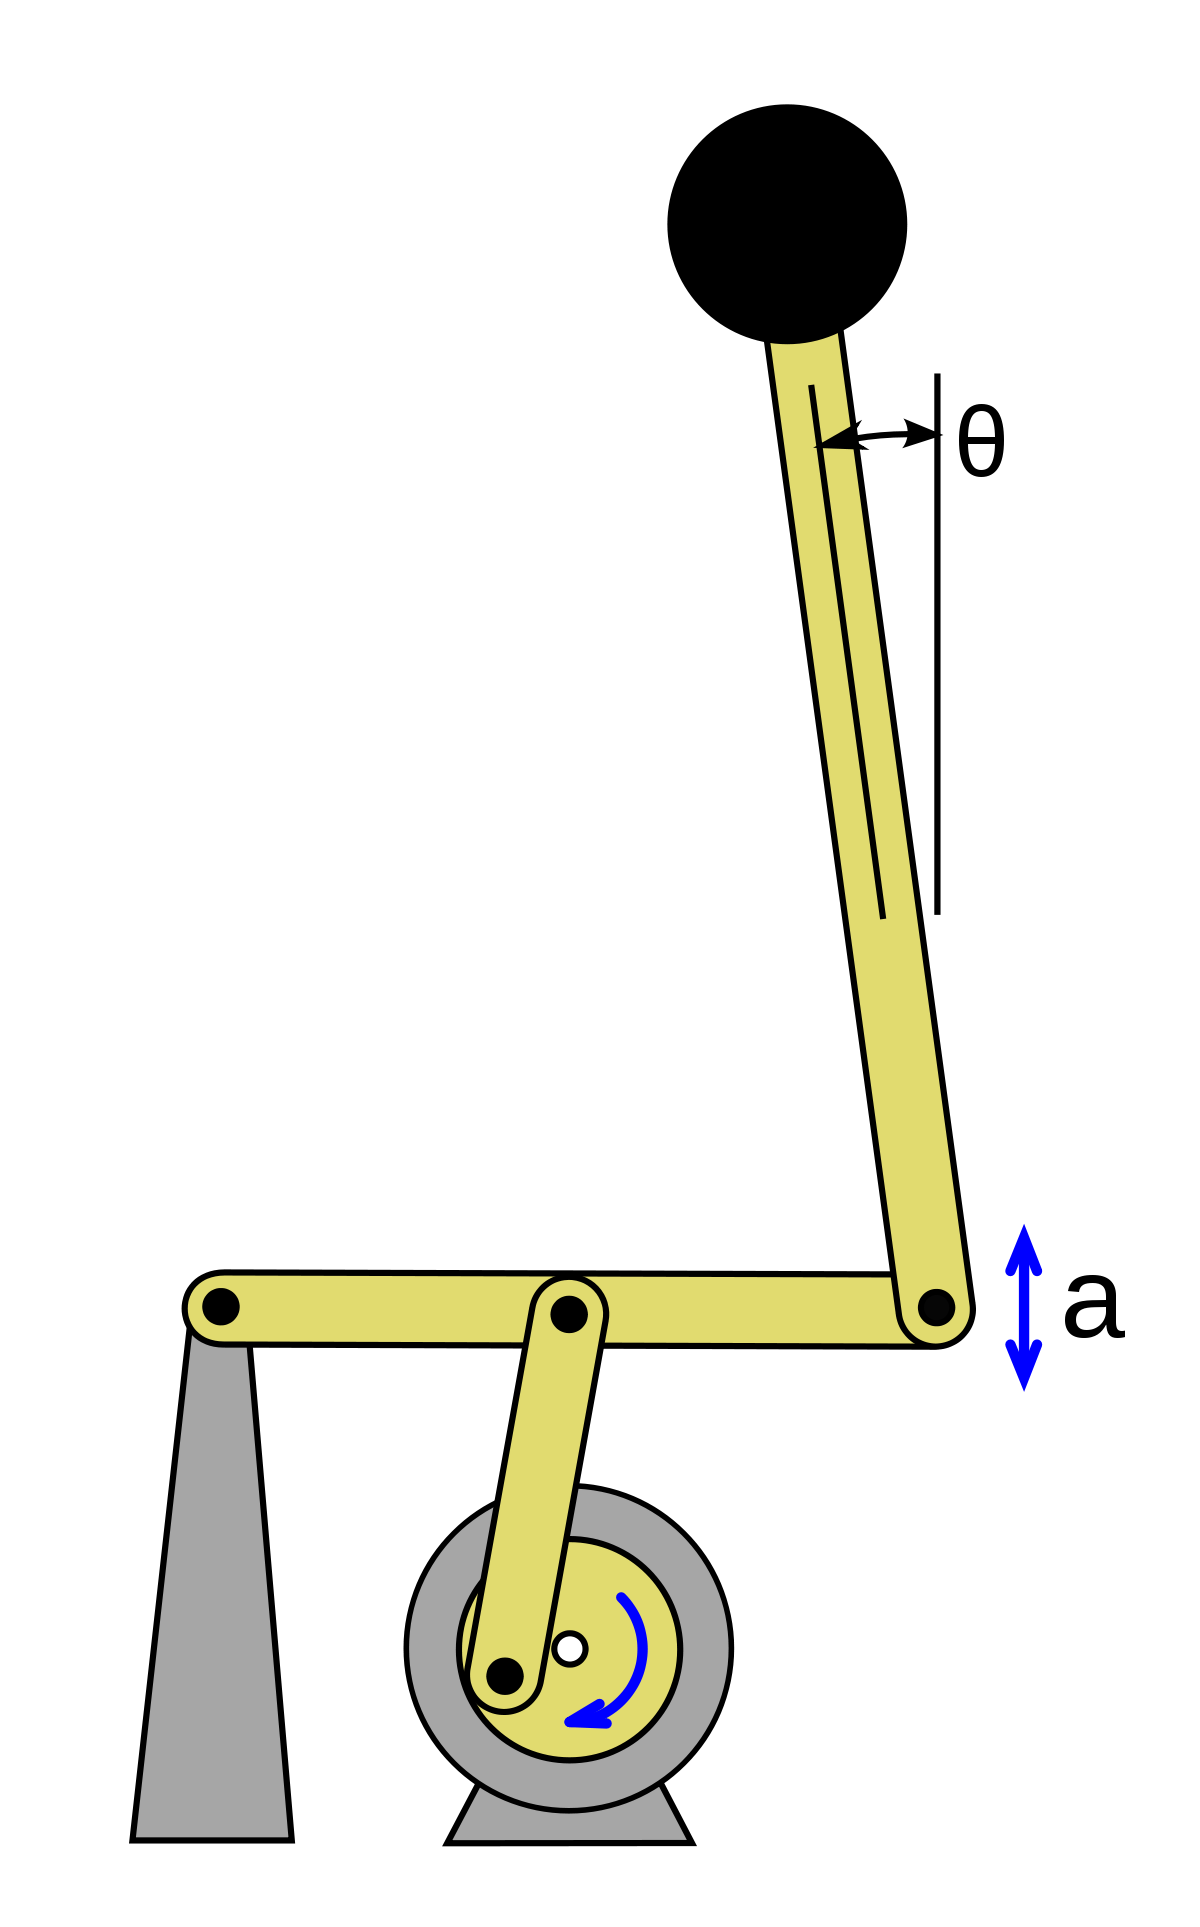
\includegraphics[scale=0.2]{sources/pend.png}
		  \end{center}
		  \vspace*{-8mm}
		  \caption{Пример конструкции маятника Капицы}\label{fig:pend}
	\end{figure}
	
	Данный маятник имеет два мехнизма, приводящие его в движение, что делает
	рисунок движения достаточно хаотичным. Существует дифференциальное 
	уравнение, описывающее движение данного маятника. Выглядит оно следующим
	образом:
	\[L\phi^{\prime\prime} + (g - A\omega^2 \sin\omega t) \sin\phi = 0.\]

	В следующих разделах с целью исследования поведения маятника при разных
	условиях будет рассматриваться именно это уравнение.

	\newpage
	\section{Выбор метода интегрирования}
	Первым вопросом, который необходимо было решить,стал выбор метода 
	интегрирования. С помощью данного метода будут построены необходимые 
	графики, и получены необходимые данные о поведении функции при различных
	начальных условиях.

	Для проведения процесса интегрирования был выбран метод Рунге-Кутта 
	четвертого порядка. Это достаточно популярный метод решения подобных 
	задач. Четвертый порядок метода позволяет получить достаточно высокую
	точность измерения данных, чтобы проводить исследования при экстремальных 
	условиях работы установки, в нашем случае это высокая амплитуда, частота
	маятника. При этом данный порядок не достаточно высок, чтобы приводить 
	к существенному усложнению вычислений и запредельному времени работы 
	программы в целом. Также, как будет проверенно в дальнейшем, данный метод
	успешно справляется с тестовой задачей, и действительно показывает 
	четвертый порядок точности при ее решении.

	Суть данного метода заключается в вычислении каждой следующей фазы 
	положения через предыдущую. При этом в процессе происходит вычисление
	четырех коэффициентов для каждой рассчитываемой величины по следующим
	формулам:

	

	\newpage
	
	\begin{thebibliography}{w:40}
		
		\bibitem{label1} Боргояков Е. А., Кособрюхова О.В. "Современные подходы в профилактике неинфекционных заболеваний". - Ачинск. - 2016.
		
	\end{thebibliography}
	
	\end{document}